\documentclass[times, utf8, seminar, numeric]{fer}
\usepackage{booktabs}
\usepackage{url}
\usepackage{float}
\usepackage{bm}

\begin{document}
	
	\nocite{*}
	
	\title{Generativno modeliranje u računalnom vidu}
	\author{Dominik Barukčić}
	\voditelj{prof. dr. sc. Tomislav Hrkać}
	
	\maketitle
	
	\tableofcontents
	
	\chapter{Uvod}
		U ovom radu obrađuje se tema generativnog modeliranja u računalnom vidu. Generativni modeli predstavljaju podskup metoda dubokog učenja koji imaju sposobnost stvaranja novih podataka sličnih onima iz stvarne domene. Takvi modeli postaju sve važniji alat u analizi i obradi slikovnih podataka jer omogućuju stvaranje realističnih slika, njihovu rekonstrukciju ili poboljšanje kvalitete te prijenos stilova i karakteristika između slika. Njihova široka primjenjivost očituje se u raznim područjima, uključujući umjetničku produkciju, medicinsku dijagnostiku, računalnu grafiku, pa čak i sigurnosne sustave. Cilj je seminarskog rada prikazati osnovne metode generativnog modeliranja, kao što su generativne suparničke mreže (GAN), varijacijski autoenkoderi (VAE) i difuzijski modeli, uz njihove primjene u području računalnog vida. Rad uključuje i praktične eksperimente korištenjem dostupnih modela te analizu rezultata generacije. Naglasak je stavljen na razumijevanje osnovnih principa svakog modela, njihovu analizu u smislu kvalitete rezultata i složenosti treniranja, kao i mogućnosti koje pružaju u stvarnim aplikacijama. 
	
	
	\chapter{Osnovni pojmovi}
		\section{Generativno modeliranje}
		Generativni model je model koji u smislu probabilističkog pristupa opisuje kako stvaramo novi skup podataka. Cilj je generativnog modeliranja izgraditi model koji što vjernije oponaša distribuciju stvarnih podataka. Kada naučimo distribuciju tih podataka, iz nje možemo uzorkovati nove različite primjere slične onima u skupu za treniranje.
		
		Pretpostavimo da imamo model koji sadrži slike automobila. Zadatak je dizajnirati model koji generira jednu novu ili skup slika automobila. To su podaci koji dosad nisu postojali, isto kao ni automobil koji bi se nalazio na generiranoj slici. Zadatak modela je naučiti pravila koja opisuju izgled automobila, tako da novi generirani uzorci budu realistični. Ovom formulacijom, opisali smo problem koji se rješava generativnim modeliranjem. 
		
		Potrebna nam je velika količina primjera objekta kojeg model treba naučiti generirati, tzv. skup za treniranje (engl. \textit{training set}). Jedan primjer iz skupa nazivamo opažanjem, ono se sastoji od velikog broja značajki. Kod slika to su najčešće vrijednosti piksela. Slike sadrže velik broj piksela, a samo manji broj kombinacija pikselnih vrijednosti čini semantički smislen sadržaj, zbog čega je problem generiranja novih slika veoma složen.
		
		Generativni model je probabilistički model. Proizvodi izlaz uzorkovan iz naučene distribucije podataka. Radi se o nedeterminističkom pristupu, što znači da ne možemo unaprijed točno znati kakav će uzorak model generirati, za razliku od determinističkih pristupa. Zbog toga model mora sadržavati stohastičku komponentu koja utječe na svaki pojedini izlaz.
		
		Zamislimo da postoji nepoznata vjerojatnosna distribucija koja opisuje kolika je vjerojatnost da se neka slika nalazi u skupu za treniranje. Gradimo model koji što vjernije oponaša tu distribuciju i omogućuje uzorkovanje novih, raznolikih uzoraka koji izgledaju poput onih iz izvorne domene.
		
		Razlikujemo dvije osnovne paradigme: \textit{diskriminativno} i \textit{generativno modeliranje}. Diskriminativno modeliranje procjenjuje uvjetnu vjerojatnost $\mathbb{P}(y \mid \mathbf{x})$, odnosno vjerojatnost da opažanje $\mathbf{x}$ pripada klasi $y$. Fokus je na učenju granice između klasa. Generativno modeliranje procjenjuje vjerojatnost $\mathbb{P}(\mathbf{x})$, koja opisuje koliko je vjerojatno opažanje $\mathbf{x}$. Ako radimo s označenim podacima, moguće je procijeniti uvjetnu vjerojatnost $\mathbb{P}(\mathbf{x} \mid y)$ koja nam opisuje koliko je vjerojatno da se opažanje $\mathbf{x}$ pojavi unutar klase $y$.
		
		
		\section{Generativna suparnička mreža}
		Generativna suparnička mreža (eng. \textit{Generative Adversarial Network}, GAN) je klasa generativnih modela koju su 2014. godine predstavili Ian Goodfellow i suradnici. GAN sadrži dvije neuronske mreže koje se treniraju u suparničkom odnosu: \textbf{generator} $G$ i \textbf{diskriminator} $D$. Cilj generatora je naučiti distribuirati podatke tako da proizvodi sintetičke uzorke $G(\bm{z})$ koji nalikuju stvarnima. Zadatak diskriminatora je razlikovati stvarne uzorke $\bm{x}$ iz skupa za treniranje od lažnih generiranih uzoraka.
		
		Generator $G$ prima slučajni vektor šuma $\bm{z}$ iz latentnog prostora i generira sintetski uzorak $G(\bm{z})$. Diskriminator $D$ nastoji maksimizirati točnost klasifikacije između stvarnih i generiranih uzoraka. Obje mreže treniraju se istovremeno, pri čemu generator pokušava zavarati diskriminator, dok diskriminator pokušava pravilno razlikovati ulaze. Proces možemo interpretirati kao minimax igru s funkcijom cilja:
		
		\[
		\min_G \max_D V(D, G) = \mathbb{E}_{\bm{x} \sim p_{\text{data}}(\bm{x})}[\log D(\bm{x})] + \mathbb{E}_{\bm{z} \sim p_{\bm{z}}(\bm{z})}[\log(1 - D(G(\bm{z})))]
		\]
		
		Idealno, ravnoteža između $G$ i $D$ dovodi do toga da se generirani podaci ne razlikuju od stvarnih, tj. $D(\bm{x}) = 0.5$ za sve ulaze. Na taj način model uči implicitnu distribuciju podataka bez potrebe za izričitom specifikacijom funkcije vjerojatnosti.
		
		\begin{figure}[H]
			\centering
			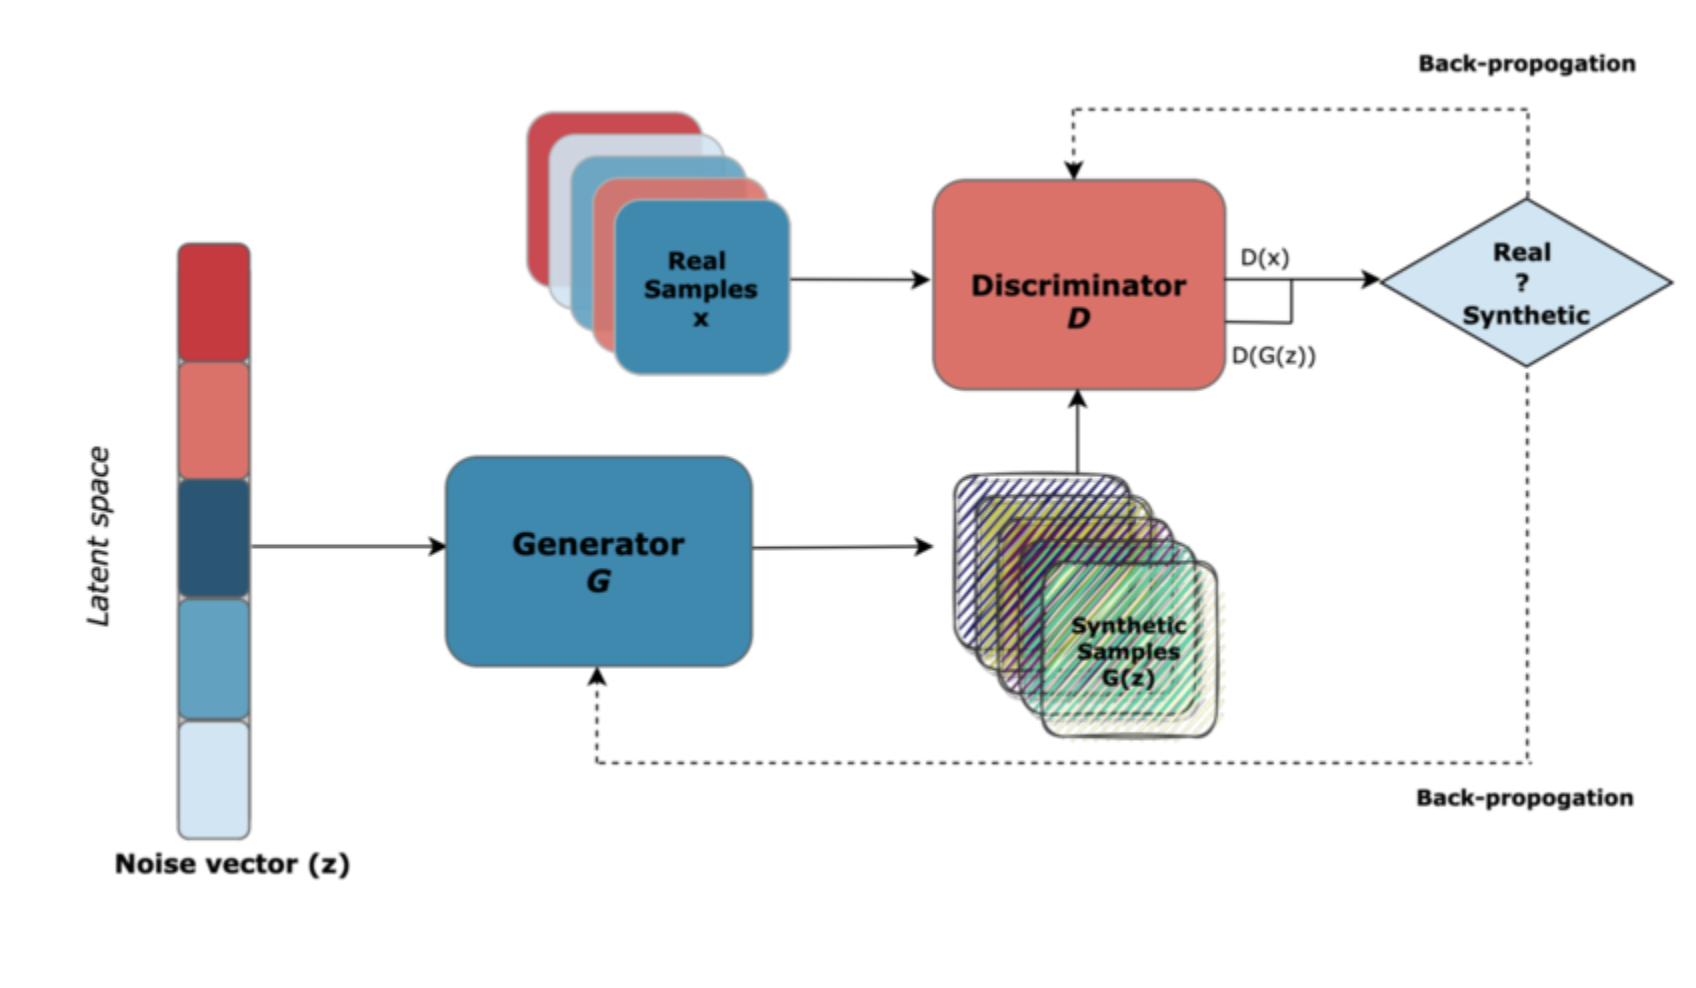
\includegraphics[width=0.9\textwidth]{images/apply/superres/GAN_shema.png}
			\caption{Shema rada generativne suparničke mreže (GAN) \cite{kinezi}}
			\label{fig:gan_arch}
		\end{figure}
		
		Kao što je istaknuto u literaturi  \cite{goodfellow2016deep} i \cite{foster2019generative}, GAN-ovi su iznimno moćni u generiranju realističnih slika, tekstura i glazbe. Važno je spomenuti da treniranje GAN-ova može biti zahtjevno. Razlozi mogu biti nestabilnost, koja se javlja zbog oscilirajuće dinamike između generatora i diskriminatora te problem \textit{mode collapse}, koji se očituje kada generator uči proizvoditi samo ograničen broj varijacija.
		
		Unatoč izazovima, GAN arhitektura temelj je mnogim modelima poput StyleGAN, CycleGAN, BigGAN, itd. Primjenjuju se u zadacima prijenosa stila, povećanja rezolucije, obradi medicinskih snimaka i u mnogim drugim primjenama.
		
		\section{Varijacijski autoenkoder}
		Autoenkoder je neuronska mreža koja se sastoji od dva dijela: enkodera i dekodera. Enkoder je dio mreže koji preslikava višedimenzionalni ulaz u reprezentacijski vektor niže dimenzije (latentni prostor). Dekoder je dio mreže koji iz latentnog vektora rekonstruira podatke natrag u izvornu domenu. Ideja je da iz latentnog prostora možemo odabrati bilo koji vektor i rekonstruirati podatak u izvornoj domeni.
		
		\begin{figure}[H]
			\centering
			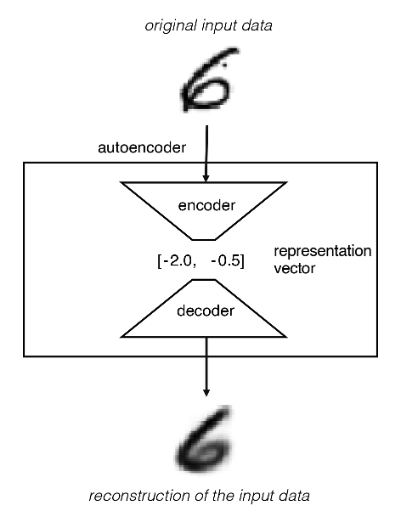
\includegraphics[width=130pt]{images/VAE/diagram_autoenc.png}
			\caption{Dijagram autoenkodera \cite{foster2019generative}}
			\label{fig:VAE}
		\end{figure}
		
		Varijacijski autoenkoder (eng. Variational Autoencoder, VAE) proširuje klasični autoenkoder tako da latentni prostor promatra probabilistički. Koristi naučeno približno zaključivanje i trenira se metodama temeljenim na gradijentnim postupcima. 
		
		\begin{figure}[H]
			\centering
			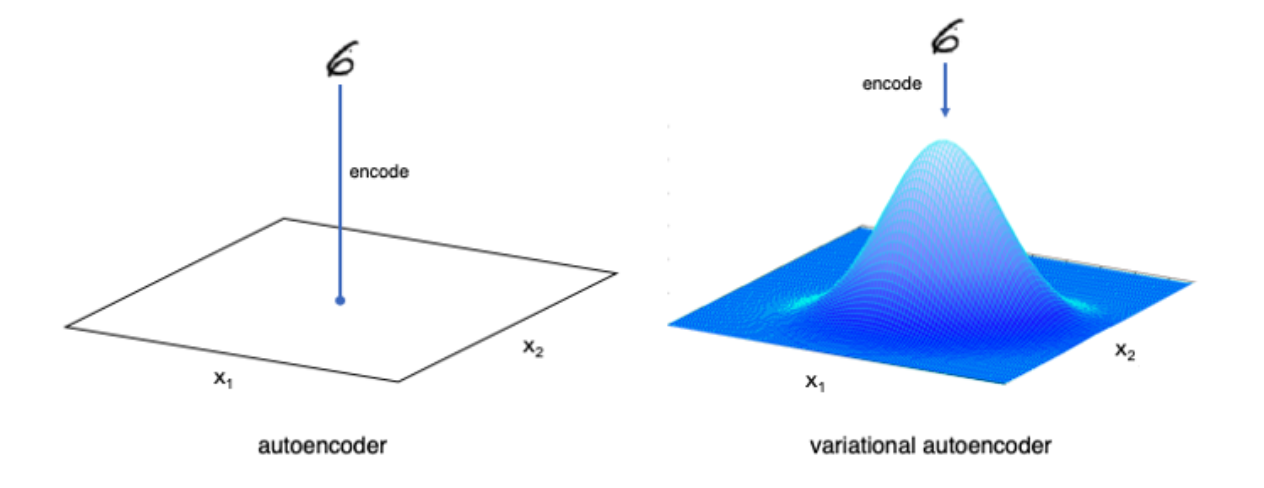
\includegraphics[width=0.75\textwidth]{images/VAE/ae_vs_vae.png}
			\caption{Razlika između autoenkodera i varijacijskog autoenkodera – deterministički vs. probabilistički prikaz latentnog prostora \cite{foster2019generative}}
			\label{fig:ae_vs_vae}
		\end{figure}
		
		Za generiranje uzorka, VAE najprije uzme uzorak $\bm{z}$ iz latentne distribucije $p_{\text{model}}(\mathbf{z})$, a trenira se maksimizacijom donje granice dokaza (eng. evidence lower bound, ELBO), definirane izrazom:
		\begin{equation}
			\mathcal{L}(q) = \mathbb{E}_{\mathbf{z} \sim q(\mathbf{z}|\mathbf{x})} \left[ \log p_{\text{model}}(\mathbf{z}, \mathbf{x}) \right] + \mathcal{H}(q(\mathbf{z}|\mathbf{x}))
			\tag{2.4.1}
		\end{equation}
		\begin{equation}
			= \mathbb{E}_{\mathbf{z} \sim q(\mathbf{z}|\mathbf{x})} \left[ \log p_{\text{model}}(\mathbf{x} | \mathbf{z}) \right] - D_{\text{KL}} \left( q(\mathbf{z}|\mathbf{x}) \,\|\, p_{\text{model}}(\mathbf{z}) \right)
			\tag{2.4.2}
		\end{equation}
		\begin{equation}
			\leq \log p_{\text{model}}(\mathbf{x})
			\tag{2.4.3}
		\end{equation}
		
		Kako bi se omogućilo propagiranje gradijenata kroz stohastički uzorak $\mathbf{z} \sim q(\mathbf{z}|\mathbf{x})$, koristi se \textbf{reparametrizacijski trik}. Umjesto direktnog uzorkivanja iz latentne distribucije, latentna varijabla $\mathbf{z}$ se izražava kao funkcija:
		
		\[
		\mathbf{z} = \bm{\mu} + \bm{\sigma} \odot \bm{\epsilon}, \quad \bm{\epsilon} \sim \mathcal{N}(0, I)
		\]
		
		gdje su $\bm{\mu}$ i $\bm{\sigma}$ parametri distribucije koje daje enkoder, a $\bm{\epsilon}$ je nezavisni slučajni šum. Postupak omogućuje izračun gradijenata kroz funkciju uzorkovanja, čime je omogućeno učenje parametara gradijentnim spustom.
		
		Funkcija gubitka sastoji se od dvije komponente:
		\begin{itemize}
			\item \textbf{Rekonstrukcijski gubitak} koji mjeri koliko dobro dekoder rekonstruira ulaz $\mathbf{x}$ iz latentne reprezentacije $\mathbf{z}$,
			\item \textbf{KL divergencija} predstavlja kaznu koja mjeri razliku između približne posteriorne distribucije $q(\mathbf{z}|\mathbf{x})$ i prethodno definirane priori distribucije $p(\mathbf{z})$, za koju obično uzimamo standardnu normalnu distribuciju.
		\end{itemize}
		
		\[
		\mathcal{L}_{\text{VAE}} = \mathbb{E}_{\mathbf{z} \sim q(\mathbf{z}|\mathbf{x})} \left[ \log p(\mathbf{x}|\mathbf{z}) \right] - D_{\text{KL}} \left( q(\mathbf{z}|\mathbf{x}) \,\|\, p(\mathbf{z}) \right)
		\]
		
		Rekonstrukcijski gubitak potiče model da uči preciznu rekonstrukciju ulaza, a KL divergencija osigurava da je latentni prostor strukturiran na način pogodan za generiranje novih uzoraka. Time je omogućena \textbf{generativna sposobnost} varijacijskog autoenkodera. Model zatim generira nove uzorke jednostavnim uzorkovanjem iz distribucije $p(\mathbf{z})$ i dekodiranjem kroz dekoder.
		
		Varijacijski autoenkoderi nalaze primjenu u zadacima poput generiranja novih slika i uzoraka, interpolacije između podataka u latentnom prostoru, uklanjanja šuma i rekonstrukcije slike te detekcije anomalija.
		
		\section{Difuzijski modeli}
		Difuzijski modeli (eng. Diffusion models) su novija klasa generativnih modela koji su iznimno učinkoviti u generiranju visoko kvalitetnih i realističnih slika. 
		Temelje se na postupku učenja generativnog procesa kroz dvije faze:
		\begin{itemize}
			\item \textbf{Difuzija} - postupno dodavanje šuma na podatke
			\item \textbf{Denoising} - postupna rekonstrukcija podataka iz šuma
		\end{itemize}
		Treniranjem model uči kako ukloniti šum iz slike, a u fazi generacije počinje od nasumičnog šuma i iterativno stvara sliku.
		
		Za razliku od GAN-ova, koji imaju probleme poput nestabilnosti u treniranju i mode collapsea, difuzijski modeli imaju veću stabilnost i visoku razlučivost generiranih uzoraka. Nedostatak im je sporo generiranje zbog velikog broja iteracija potrebnih za postupno uklanjanje šuma.
	
	
	\chapter{Primjene u računalnom vidu}		
		Zahvaljujući sposobnosti stvaranja realističnih i korisnih vizualnih podataka, generativni modeli imaju široku primjenu u računalnom vidu. U nastavku su opisane sljedeće primjene.
		
		\section{Generiranje sintetičkih slika}
		Strmoglavim razvojem područja pojavljuju se zahtjevi za velikom količinom kvalitetnih podataka. Model je onoliko dobar koliko su i podaci koje koristimo za treniranje i validaciju. Prikupljanje takvih podataka u praksi ispada vremenski zahtjevno, a time i skupo. Ako tome dodamo zakonska ograničenja, dolazimo do još većih poteškoća (npr. GDPR, etika u medicini ili nadzornoj sigurnosti). Jedno od rješenja jest generiranje sintetičkih podataka. U tu svrhu možemo koristiti bilo koji generativni model ili kombinaciju s alatima jezgara igre (eng. game engine) ili 3D modeliranja. \cite{jimaging8110310}
		
		
		Sintetičke slike možemo klasificirati u dvije glavne kategorije:
		\begin{itemize}
			\item \textbf{Složene (kompozitne) slike} - kombinacija stvarnih pozadina s različitim objektima
			\item \textbf{Potpuno virtualne slike} - generirane u potpunosti
		\end{itemize}
		
		
		Sintetički podaci mogu dopuniti ili proširiti stvarne skupove. Također, možemo im smanjiti pristranost ili izbaciti neke skupe realne podatke. GAN modeli su kvalitetni u generiranju slika lica, a velika je korist što ne narušavamo tuđu privatnost ili sigurnost. Postoje drugi modeli koji služe za simuliranje 3D okruženja kojima možemo testirati teške uvjete bez stvarnog rizika. Mogućnosti su brojne, ali ne dolaze bez plaćanja cijene. \cite{jimaging8110310}
		
		\textbf{Prednosti: }
		\begin{itemize}
			\item automatizirano označavanje podataka
			\item skalabilnost i kontrola
			\item očuvanje privatnosti i sigurnosti
		\end{itemize}
		
			\textbf{Nedostaci: }
		\begin{itemize}
			\item često sintetički podaci imaju lošije rezultate u odnosu na realne 
			\item zahtjevni računalni resursi
			\item nema univerzalne metodologije za ocjenu kvalitete podataka
		\end{itemize}
		
		\begin{figure}[H]
			\centering
			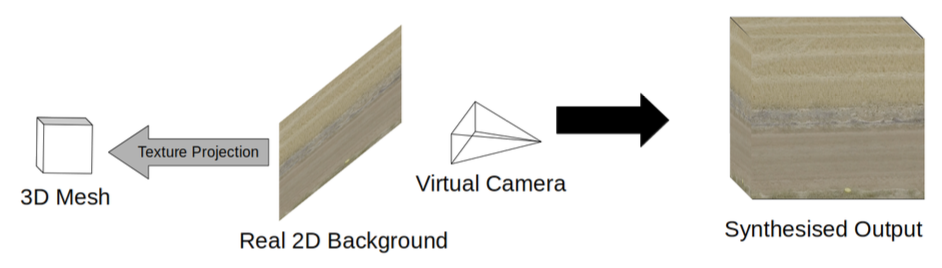
\includegraphics[width=300pt]{images/apply/synthetic/synthetic_data.png}
			\caption{Sinteza projekcijom stvarne 2D slike na 3D mrežu \cite{jimaging8110310}}
			\label{fig:synthetic}
		\end{figure}
		
		\section{Povećanje rezolucije}
		Povećanje rezolucije slike (eng. Super-resolution) problem je u računalnom vidu kojim nastojimo iz ulazne slike niske razlučivosti generirati sliku visoke razlučivosti. Dostupne su klasična metode interpolacije, ali ne pružaju nikakve nove informacije. Metode generativnog modeliranja, posebice generativne suparničke mreže, omogućuju učenje distribucija visokih razlučivosti u cilju nadopune izgubljenih detalja. 
		
		GAN pristupi za povećanje rezolucije sastoje se od 2 modela:
		\begin{itemize}
			\item \textbf{Generatora} koji generira visoko-razlučivu sliku iz nisko-razlučivog ulaza
			\item \textbf{Diskriminatora} koji razlikuje generiranu sliku od stvarne visoko-razlučive slike
		\end{itemize}
		Diskriminator kao suparnički proces generatoru, omogućuje da s vremenom poboljša kvalitetu generiranih slika kako bi zavarale diskriminator.
		
		Metode možemo klasificirati prema vrsti učenja:
		\begin{itemize}
			\item \textbf{Polunadzirano učenje} - kombinira ograničene označene podatke s velikim brojem neoznačenih podataka
			\item \textbf{Nenadzirano učenje} - koristi samo neoznačene podatke, često uz dodatne tehnike poput cikličke konzistencije
		\end{itemize}
		
		Neki istaknuti GAN modeli za super-rezoluciju:
		\begin{itemize}
			\item \textbf{SRGAN} -  prvi GAN model za super-rezoluciju koji koristi perceptualnu funkciju gubitka za generiranje vizualno uvjerljivih slika
			\item \textbf{ESRGAN} - poboljšanje SRGAN-a koje uvodi Residual-in-Residual Dense Block (RRDB) za bolju rekonstrukciju detalja i koristi relativistički pristup u diskriminatoru
			\item \textbf{Real-ESRGAN} - proširenje ESRGAN-a koje se fokusira na stvarne degradacije slika, omogućujući bolje rezultate na slikama iz stvarnog svijeta
		\end{itemize}
		
		
		Prilikom treniranja, dostupne su različite funkcije gubitaka:
		\begin{itemize}
			\item \textbf{Adversarijalni gubitak} - potiče generator da stvara slike koje su teško razlikovljive od stvarnih
			\item \textbf{Perceptualni gubitak} - koristi značajke iz unaprijed treniranih mreža (npr. VGG) za očuvanje vizualnih karakteristika
			\item \textbf{Funkcija gubitka sadržaja} - mjeri razliku između generirane i stvarne slike na pikselnoj razini
		\end{itemize}
		
		Evaluacija performansi modela provodi se pomoću metrika kao što su PSNR (Peak Signal-to-Noise Ratio) i SSIM (Structural Similarity Index), iako ove metrike ne koreliraju uvijek s percepcijskom kvalitetom slike.
		
		\section{Prijenos stila}
		Prijenos stila (eng. Style transfer) tehnika je kojom se sadržaj slike (npr. boje, teksture, debljina kista) prenosi na drugu sliku, zadržavajući stil originalne slike. Generativni modeli, specifično GAN-ovi, iznimno su učinkoviti u ovoj domeni. Osnovni cilj je generirati sliku koja zadržava semantički sadržaj originalne slike vizualno oblikovan prema ciljnom stilu. Primjene su u umjetnosti, produkciji, animaciji, društvenim mrežama i medicinskoj vizualizaciji.
		Tri istaknuta pristupa prijenosu stila temeljena na GAN arhitekturi - CycleGAN, StyleGAN i TL-GAN - analizirana su u radu Bo i sur. \cite{bo2021style}
		
		Svaki od ovih modela koristi različite arhitekture i strategije za prijenos stila:
		\begin{itemize}
			\item \textbf{CycleGAN} omogućuje stilizaciju između dviju domena bez uparenih primjera koristeći cikličku konzistenciju.
			\item \textbf{StyleGAN} uvodi mapirajuću mrežu i višestupanjsko umetanje latentnog vektora, tako postiže bolju kontrolu nad generiranim stilovima.
			\item \textbf{TL-GAN} omogućuje preciznu kontrolu nad atributima slike kombiniranjem pretreniranih klasifikatora s GAN-ovima, bez potrebe za ponovnim treniranjem generatora.
		\end{itemize}
		
		Idealni model za prijenos stila treba omogućiti:
		\begin{itemize}
			\item Preciznu kontrolu stilskih atributa
			\item Efikasnost treniranja i izvedbe
			\item Skalabilnost na slike visoke rezolucije
			\item Mogućnost integracije s detektorima objekata radi selektivne primjene stila
			\item Naknadnu optimizaciju rezultata radi korekcije neželjenih deformacija
		\end{itemize}
		
		\section{Uklanjanje šuma}
		Uklanjanje šuma sa slika (eng. denoising) jedan je od klasičnih zadataka u računalnom vidu gdje model mora naučiti rekonstruirati izvornu sliku iz njezine oštećene verzije. Denoising autoencoder (DAE) predstavlja robusnu arhitekturu neuronske mreže dizajniranu kako bi se spriječila prenaučenost (eng. overfitting) i potaknulo učenje korisnih značajki za dobru generalizaciju modela.
		
		Denoising autoencoder, predstavili su Vincent i suradnici 2008. godine. Za razliku od klasičnog autoenkodera koji pokušava naučiti funkciju identiteta, DAE uzima šumom kontaminiran ulaz i trenira mrežu tako da rekonstruira prvobitni ulaz. \cite{weng2018VAE}
		
		\begin{figure}[H]
			\centering
			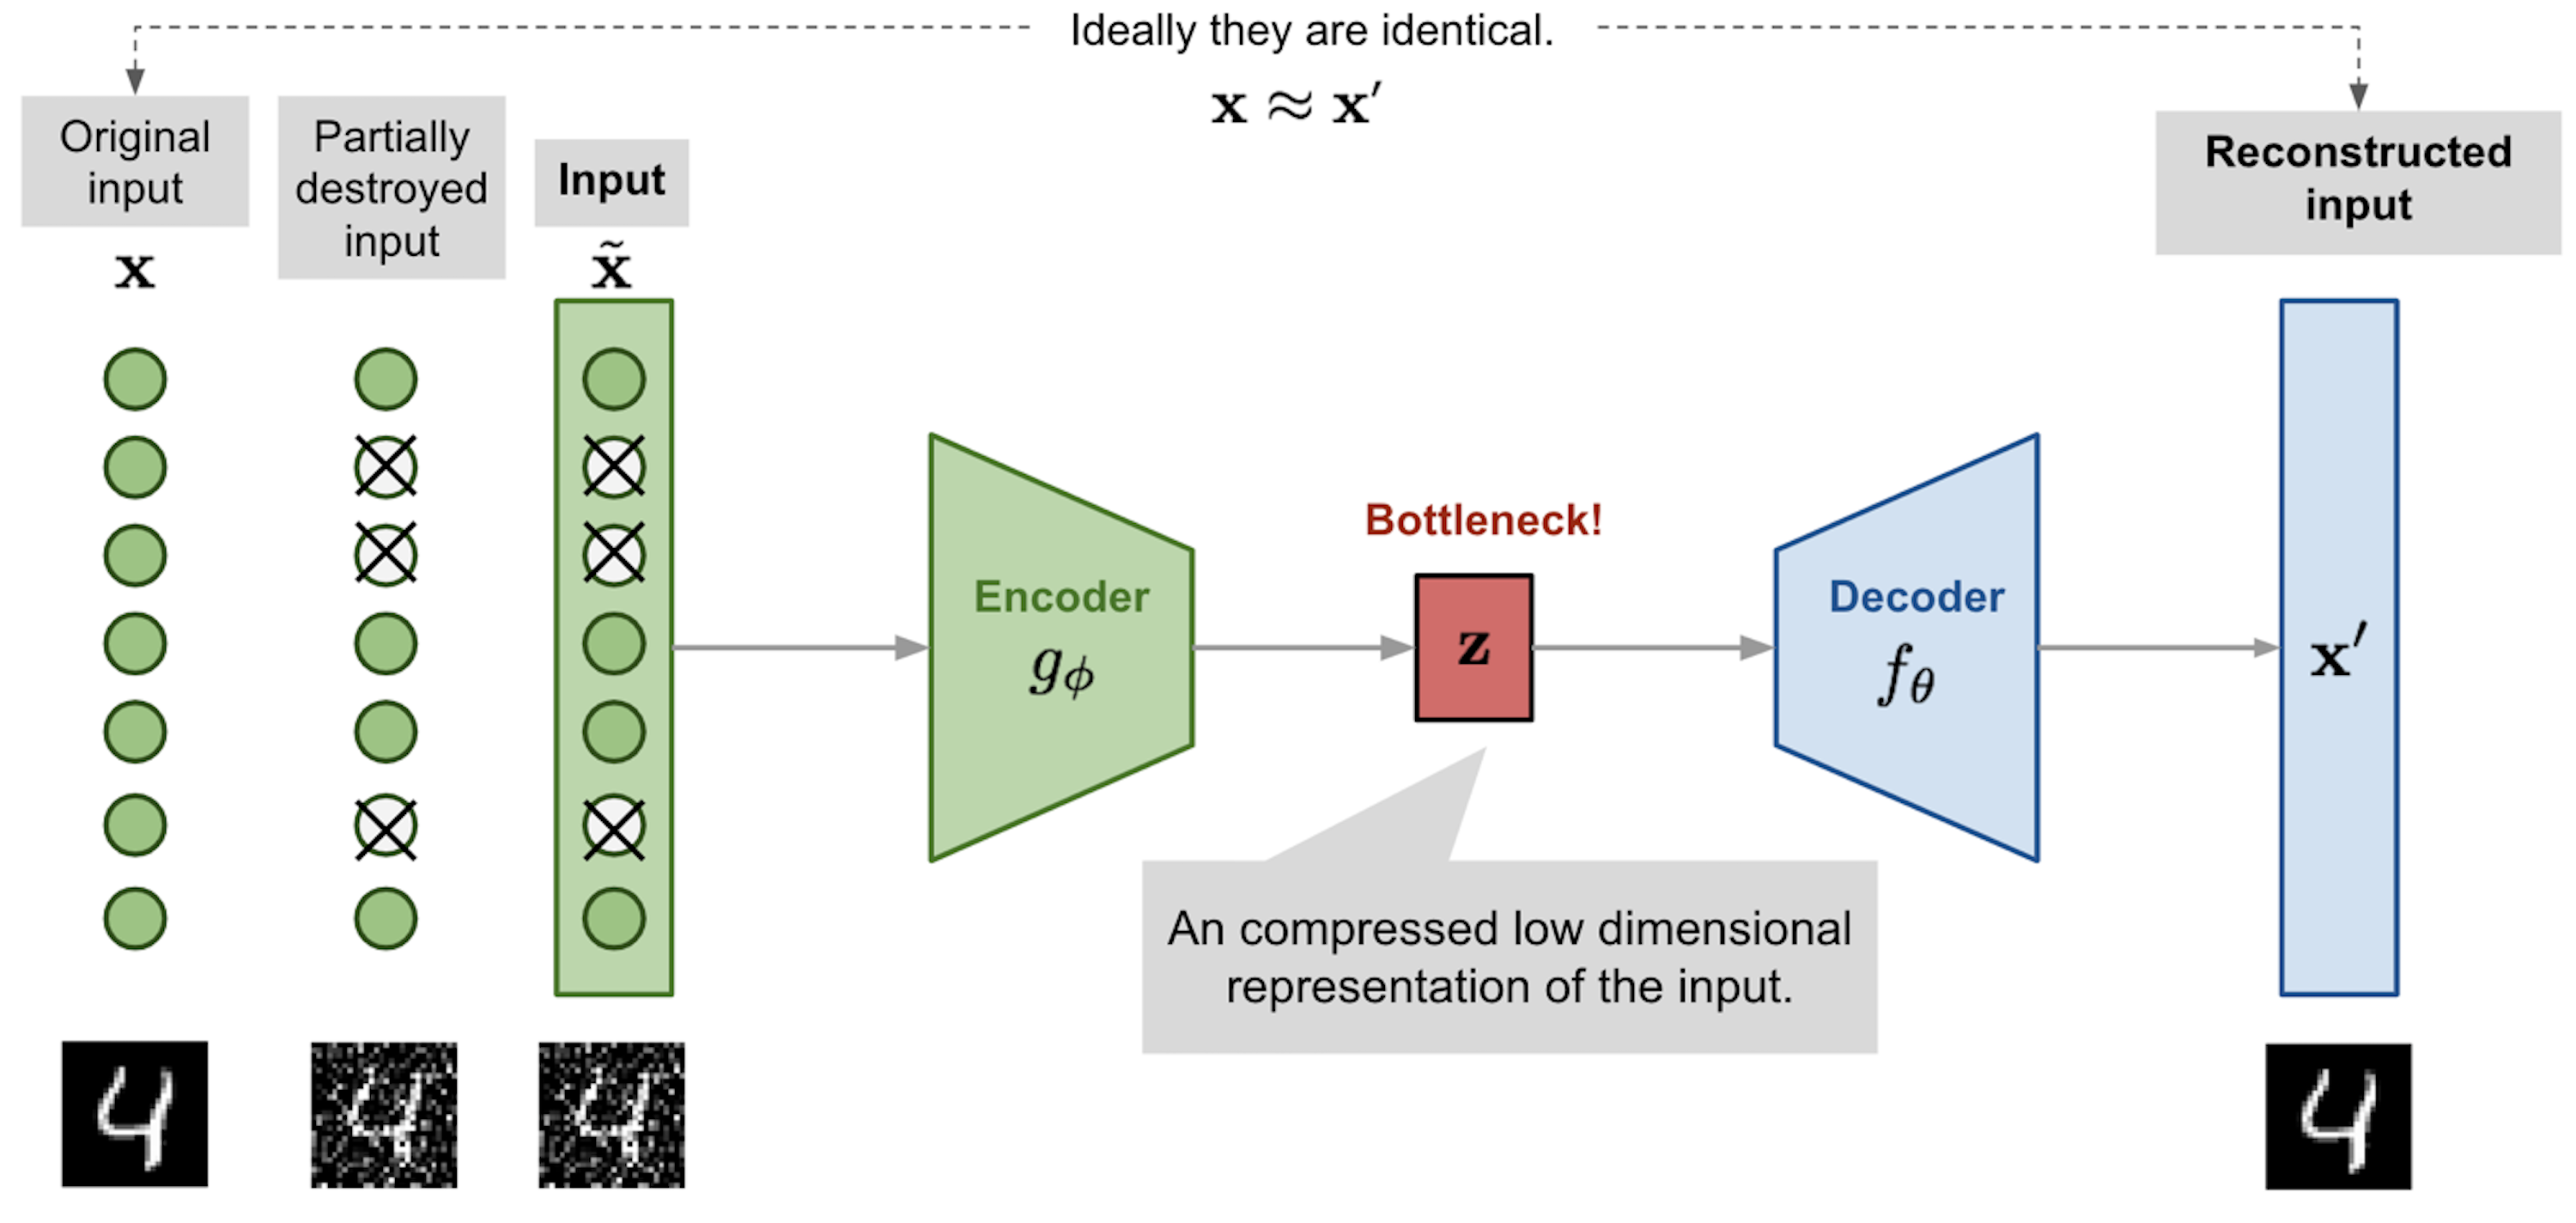
\includegraphics[width=0.8\textwidth]{images/apply/denoising/dae_diagram.png}
			\caption{Arhitektura autoenkodera za uklanjanje šuma \cite{weng2018VAE}}
			\label{fig:dae}
		\end{figure}
		
		Prilikom treniranja, ulazne slike se kontaminiraju različitim vrstama šuma (npr. Gaussov, "salt and pepper", zamračenje piksela). Model tada uči rekonstrukciju izvorne, čiste slike. Cilj je da mreža ne pamti šablone, nego da nauči relevantne apstraktne značajke koje pomažu u oporavku slike.
		
		Takav pristup ima dvostruku korist:
		\begin{itemize}
			\item \textbf{Robusnost} - otpornost na male varijacije i šum u ulazu
			\item \textbf{Generalizacija} - lakše učenje strukturalnih odnosa između piksela i ne oslanjanje na pojedinačne vrijednosti
		\end{itemize}
		
		Izvorni eksperiment uključivao je maskiranje piksela (nasumično postavljanje dijela ulaznih vrijednosti na nulu). Primijetimo kako ovo podsjeća na dropout, iako je DAE predstavljen 4 godine prije dropout tehnike. \cite{weng2018VAE}
		
		Kod visokodimenzionalnih podataka (npr. slika), ova metoda omogućuje modelu da:
		\begin{itemize}
			\item nauči ovisnosti između piksela
			\item raspozna semantičke informacije iz nepotpunih ulaza
			\item poboljša stabilnost i robusnost latentnog prostora
		\end{itemize}
		
		Kombinacija DAE sa varijacijskim autoenkoderom (VAE) proširuje mogućnosti. Model osim uklanjanja šuma, koristi probabilistički latentni prostor kako bi omogućio generativne mogućnosti.
		
	
	\chapter{Praktični eksperiment}
		\section{Generiranje sintetičke slike lica korištenjem StyleGAN}
		Za generiranje realističnih slika lica korišten je model StyleGAN3-R, kojeg je razvila NVIDIA. Treniran je na skupu FFHQ (Flickr-Faces-HQ) koji sadrži slike visoke kvalitete ljudskih lica u rezoluciji od 1024×1024 piksela. StyleGAN3 predstavlja značajno poboljšanje u odnosu na prethodne verzije (StyleGAN i StyleGAN2) jer rješava problem aliasinga i omogućuje glatke interpolacije u latentnom prostoru.
		
		Model je preuzet sa službenog NVIDIA repozitorija te lokalno pokrenut korištenjem Pythona i biblioteke PyTorch. Generiranje se temelji na uzorkovanju latentnog vektora $\bm{z}$ iz višedimenzionalnog Gaussovog prostora, koji se potom prosljeđuje kroz generativnu mrežu (inferencija). Rezultat je slika visoke rezolucije koja prikazuje lice osobe koje zapravo ne postoji.
		
		Proces generiranja prikazan je u nastavku:
		\begin{itemize}
			\item Učitavanje pretreniranog modela \texttt{stylegan3-r-ffhq-1024x1024.pkl}
			\item Generiranje latentnog vektora slučajnim uzorkovanjem iz $N(0, I)$
			\item Prolazak latentnog vektora kroz mrežu i dobivanje slike
		\end{itemize}
		
		Dobivena slika prikazana je na slici \ref{fig:stylegan3_generated}.
		
		\begin{figure}[H]
			\centering
			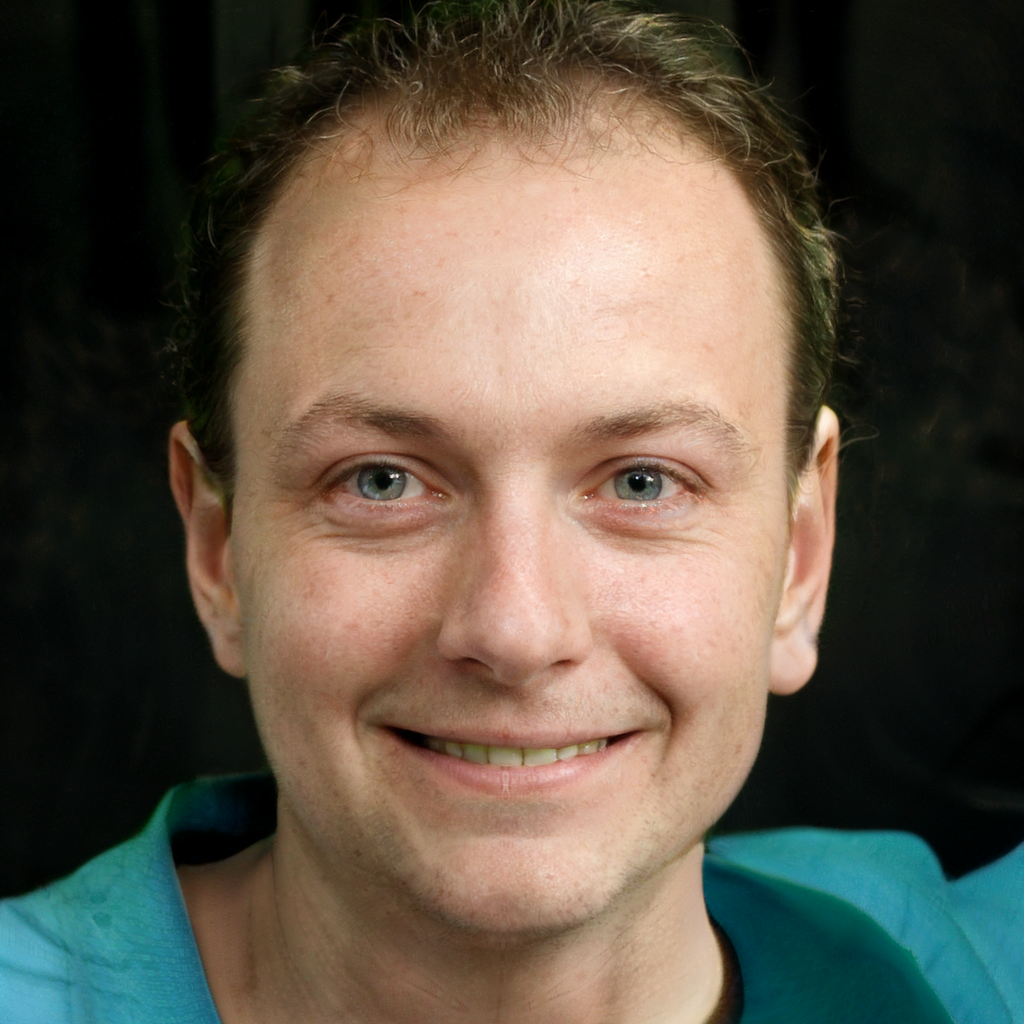
\includegraphics[width=0.3\textwidth]{images/experiment/generation/generated_face.png}
			\caption{Generirana slika lica}
			\label{fig:stylegan3_generated}
		\end{figure}
		
	\section{Povećanje rezolucije korištenjem Real-ESRGAN}
	Za eksperiment povećanja rezolucije korišten je pretrenirani model Real-ESRGAN (Real-Enhanced Super-Resolution Generative Adversarial Network). To je unaprijeđena verzija ESRGAN-a dizajnirana za bolje generaliziranje nad realističnim slikama. Model koristi RRDB (Residual-in-Residual Dense Block) arhitekturu i sposoban je rekreirati izgubljene detalje i oštrinu u slikama niske kvalitete.
	
	Korišten je model \texttt{RealESRGAN\_x4plus}, preuzet iz službenog repozitorija\newline\texttt{xinntao/Real-ESRGAN} i pokrenut lokalno na CPU-u. Budući da FP16 preciznost nije podržana na CPU-u, korišten je parametar \texttt{--fp32}, uz \texttt{--tile 128} za optimizaciju memorijske potrošnje. \cite{wang2021realesrgan}
	
	Eksperiment je proveden na slici u niskoj rezoluciji prikazujući sliku grada Zagreba iz davnina. Cilj je bio povećati razlučivost i istovremeno rekonstruirati oštrinu i detalje koji su izgubljeni zbog degradacije.
	
	Rezultati eksperimenta prikazani su na slici \ref{fig:real_esrgan_result}.
	
	\begin{figure}[H]
		\centering
		\begin{minipage}{0.45\textwidth}
			\centering
			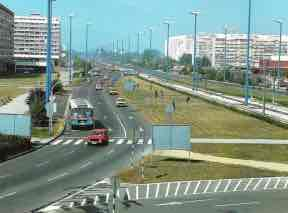
\includegraphics[width=\linewidth]{images/experiment/superresolution/zagreb.jpg}
			\caption*{Izvorna slika niske razlučivosti}
		\end{minipage}
		\hfill
		\begin{minipage}{0.45\textwidth}
			\centering
			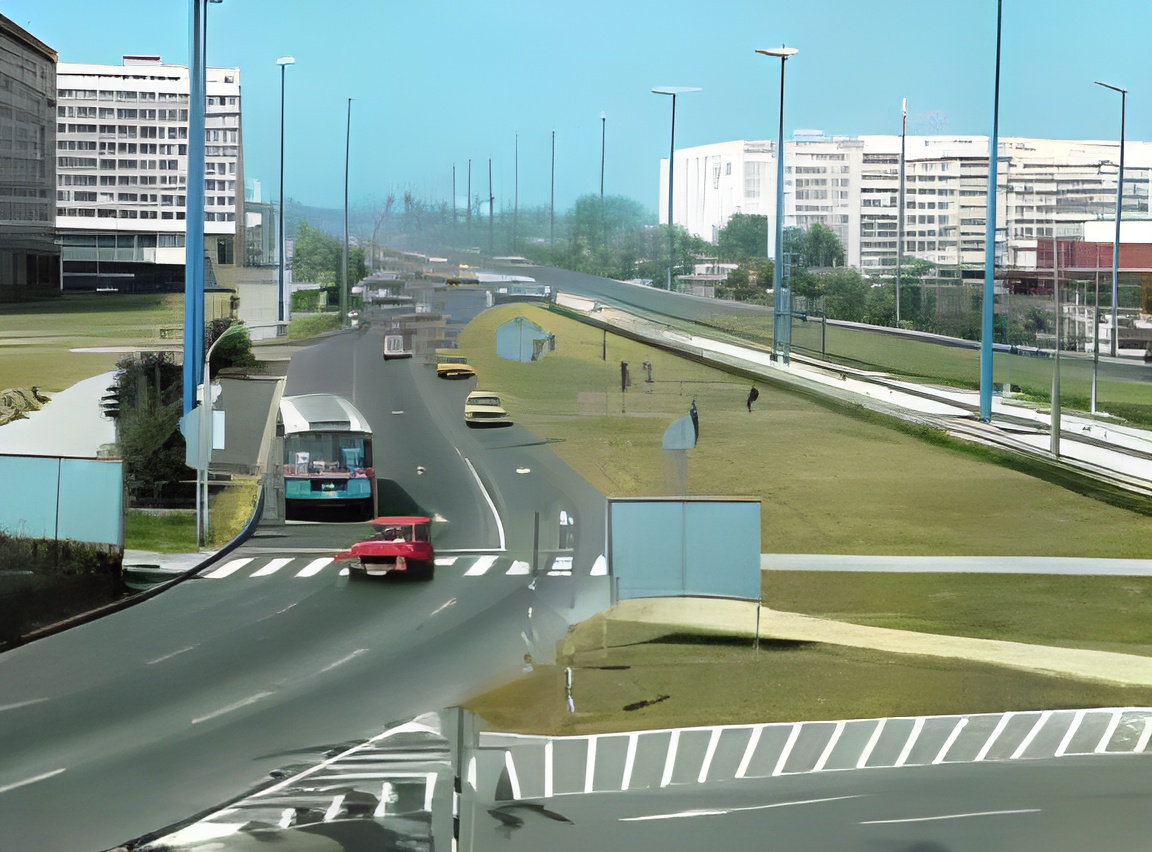
\includegraphics[width=\linewidth]{images/experiment/superresolution/zagreb_out.jpg}
			\caption*{Generirana slika visoke razlučivosti}
		\end{minipage}
		\caption{Rezultati povećanja rezolucije korištenjem Real-ESRGAN modela}
		\label{fig:real_esrgan_result}
	\end{figure}
	
	Model je uspješno poboljšao vizualnu jasnoću slike. Povećao je oštrinu na prometnim znakovima, rubovima zgrada te linijama ceste. Model je donekle rekonstruirao izgubljene teksture i eliminirao dio kompresijskih artefakata, iako se mogu primijetiti manja iskrivljenja u područjima gdje nedostaje dovoljno informacija u izvornim pikselima. Ovo je veoma korisno za obnovu starih fotografija ili unapređenje ulaznih podataka za računalni vid (npr. detekcija objekata).
	
	\section{Prijenos stila korištenjem CycleGAN}
	Za potrebe eksperimenta korišten je pretrenirani CycleGAN model za prijenos stila iz umjetničkog stila Claudea Moneta u domenu realističnih fotografija pejzaža (model \texttt{monet2photo}). \cite{CycleGAN2017}
	
	\begin{figure}[H]
		\centering
		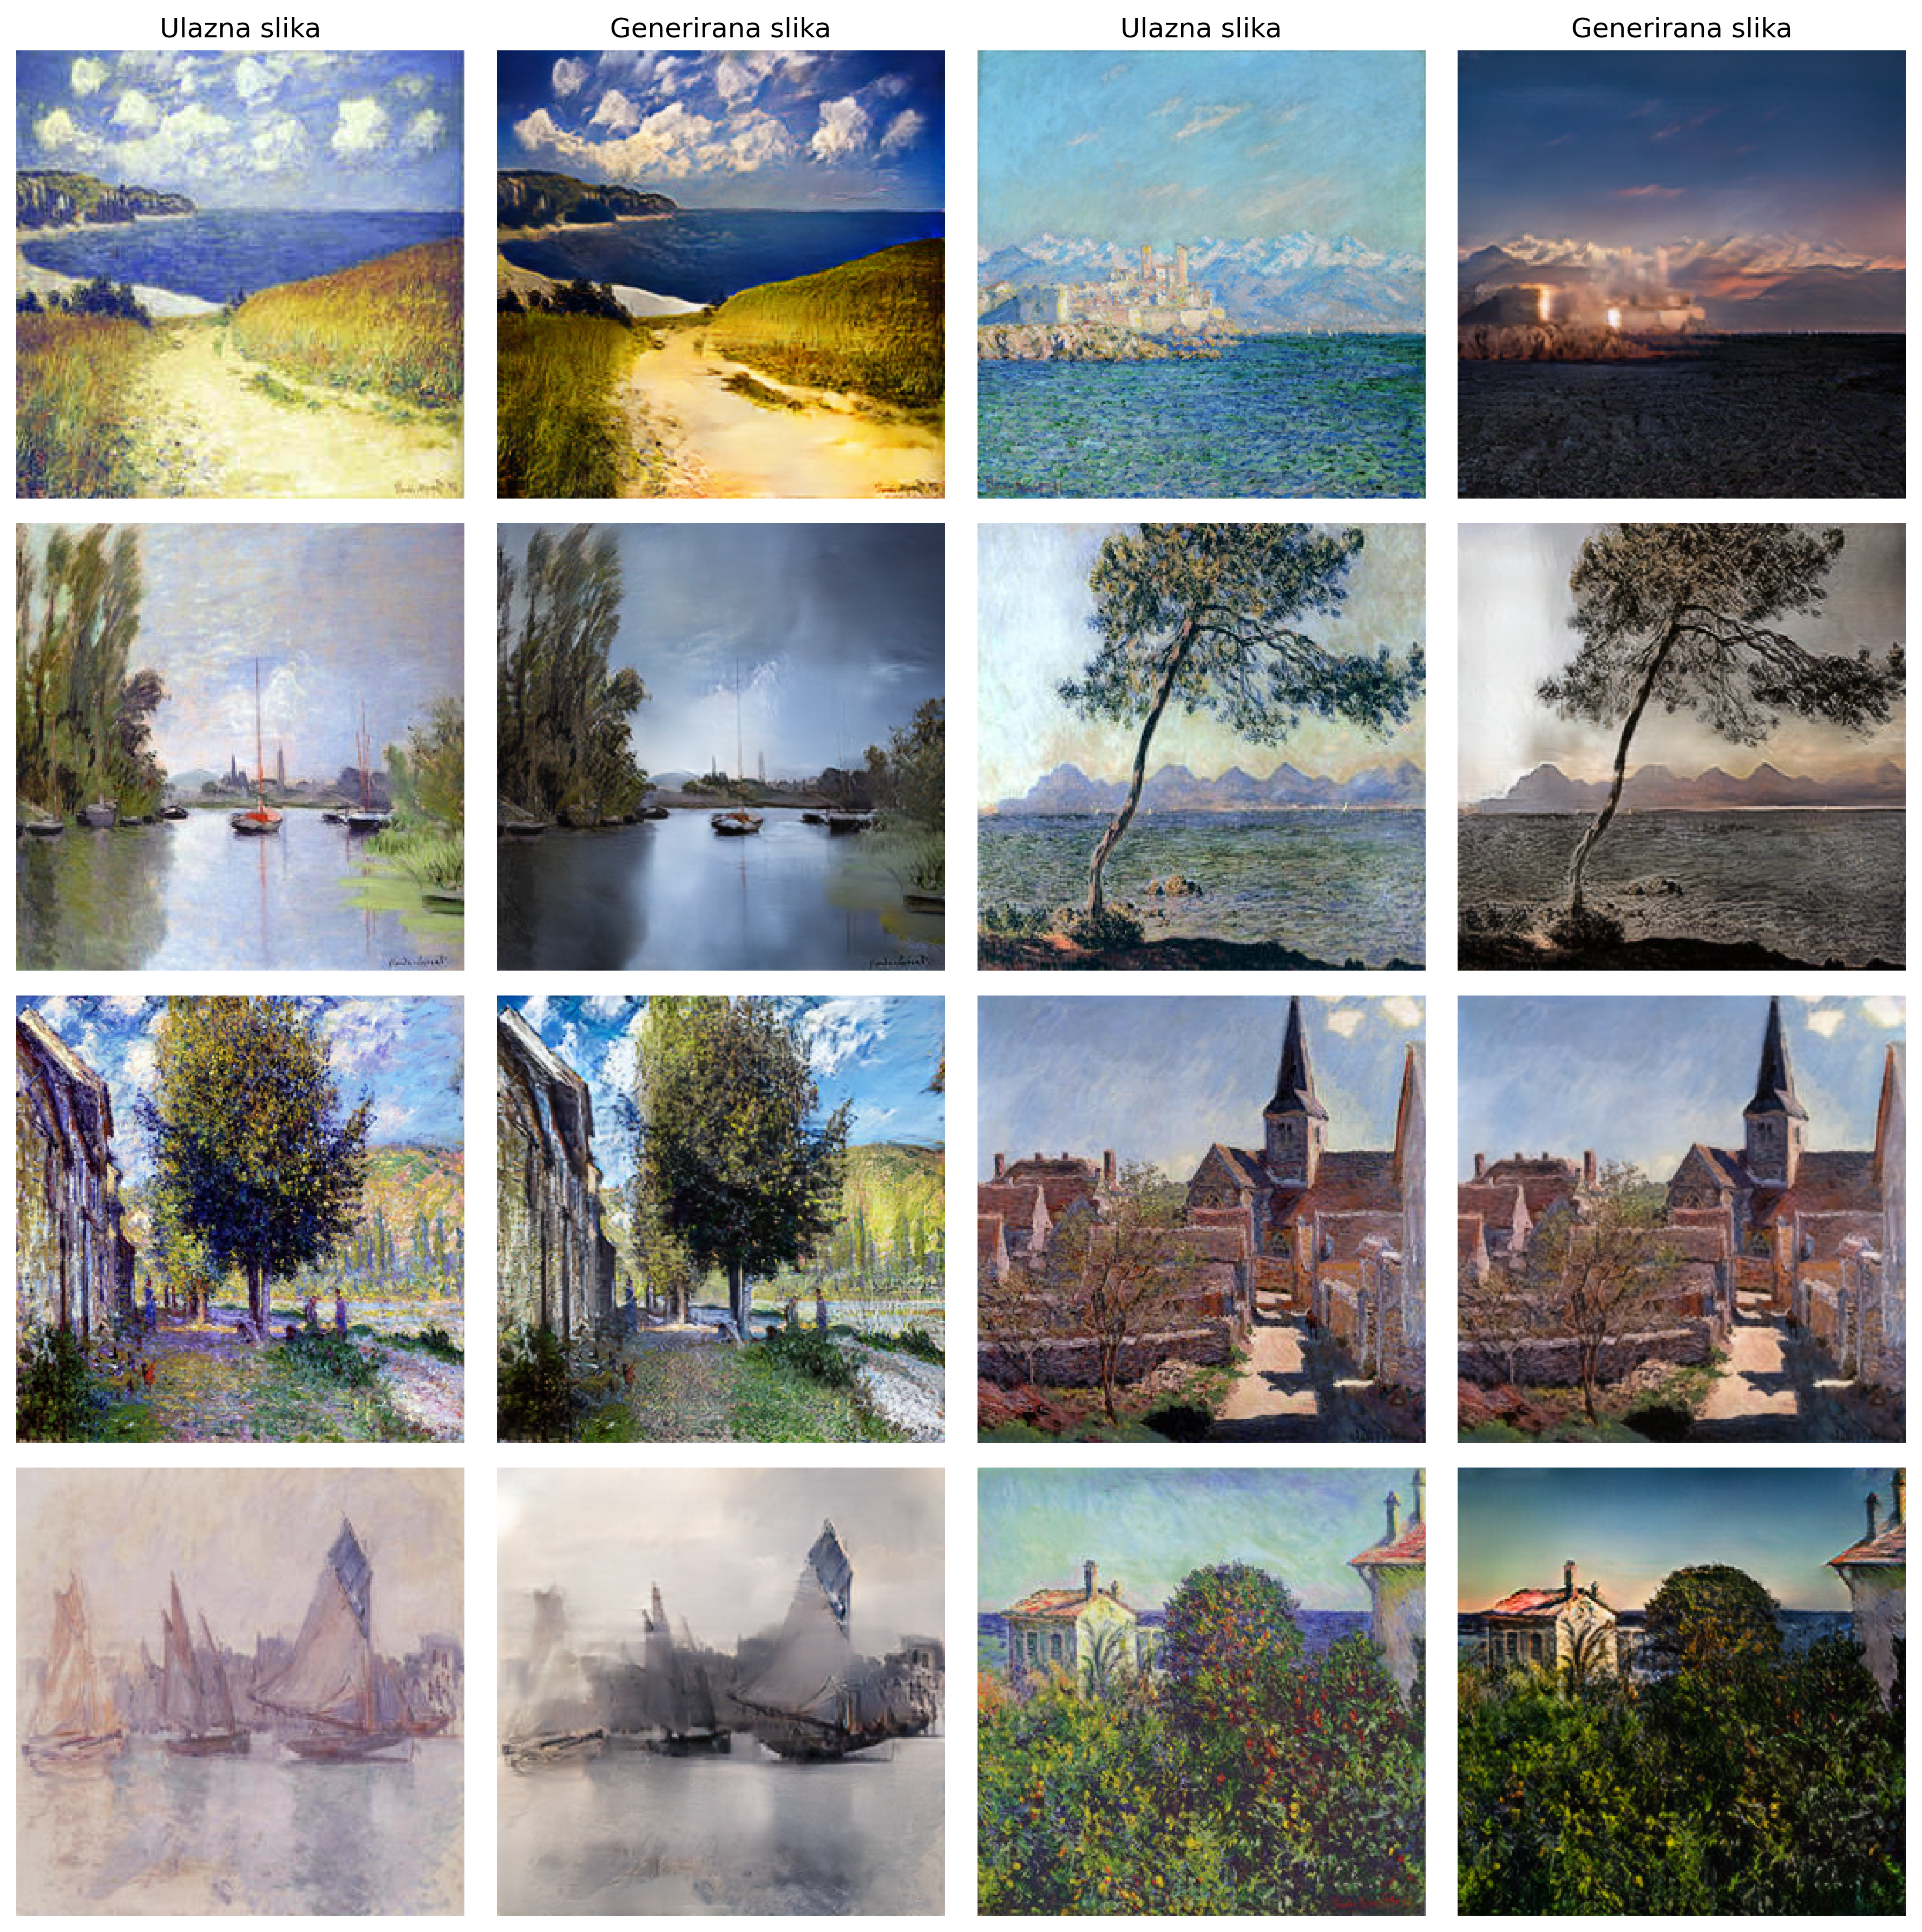
\includegraphics[width=0.72\textwidth]{images/experiment/style/monet2photo.png}
		\caption{Prijenos stila: Monetova slika (lijevo) i generirani realistični pejzaž (desno)}
	\end{figure}
	
	Rezultati generiranja prikazani na slici pokazuju različite stupnjeve uspješnosti prijenosa stila iz Monetovog umjetničkog izraza u fotorealistični prikaz. U prva dva retka možemo primijetiti uspješnu transformaciju gdje su generirane slike zadržale semantičku strukturu ulazne slike uz realistični efekt prijenosa stila. Kod određenih primjera razlike između ulazne i generirane slike su minimalne ili teško uočljive. U takvim slučajevima model očito nije dovoljno dobro "prepoznao" koje elemente treba transformirati, što može biti posljedica:
	\begin{itemize}
		\item nedostatne razlike između stilova iz skupa za treniranje
		\item ograničenja modela u generalizaciji na određene kompozicije
		\item nedostatka informacija o dubini ili strukturi scene u slici
	\end{itemize}
	
	Primjećujemo da model bolje funkcionira na slikama s jasnim kompozicijama, kontrastima i osvjetljenjem, dok slike s difuznijim konturama i teksturama zadržavaju više karakteristika Monetovog stila iako bi trebale biti realističnije. Zaključujemo da model pokazuje sposobnost prijenosa stila, ali rezultati nisu u svim slučajevima konzistentni te ovise o karakteristikama ulazne slike.

	\section{Uklanjanje šuma korištenjem VAE}
		U ovom eksperimentu korišten je varijacijski autoenkoder (VAE) za uklanjanje šuma s rukom pisanih znamenki iz skupa MNIST. Model je treniran tako da iz slike s dodatnim Gaussovim šumom nauči rekonstruirati originalnu i čistu inačicu slike. VAE koristimo kao denoising autoencoder koji je specijalizirana arhitektura za obradu degradiranih slika. \cite{weng2018VAE}
		
		Podaci su prethodno normalizirani i prošireni šumom s Gaussovom distribucijom, nakon čega treniramo model kojemu su ulazne slike one s dodanim šumom, a ciljne slike su originali. Model koristi konvolucijske slojeve u enkoderu i dekoderu te latentni prostor dimenzije 128.
		
		Rezultati su prikazani na slici \ref{fig:vae_denoising} i sastoje se od tri reda:
		\begin{itemize}
			\item Original - originalne slike iz skupa MNIST
			\item Noisy - slike s dodatnim šumom
			\item Denoised - slike rekonstruirane pomoću VAE-a
		\end{itemize}
		
		\begin{figure}[H]
			\centering
			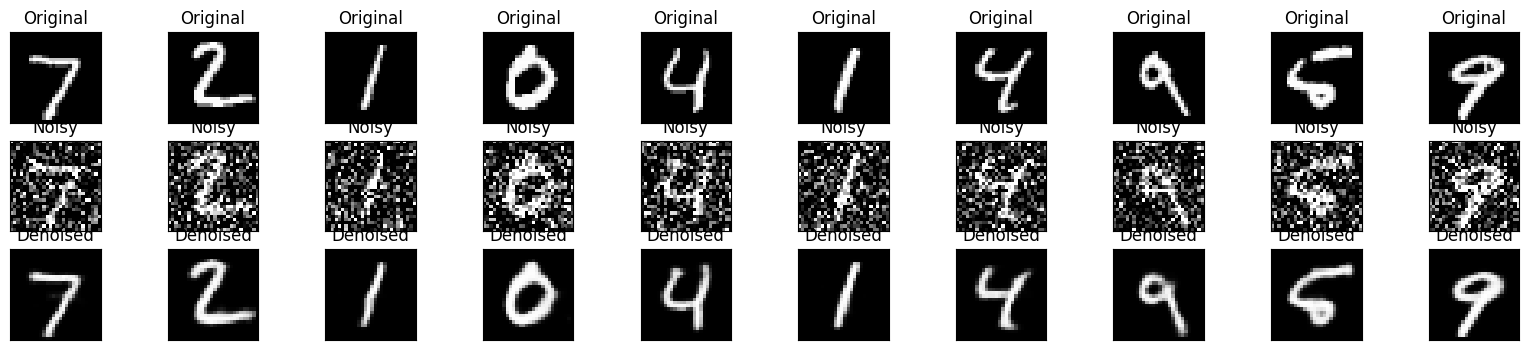
\includegraphics[width=\textwidth]{images/experiment/denoising/vae_denoising.png}
			\caption{Uklanjanje šuma s MNIST slika pomoću varijacijskog autoenkodera}
			\label{fig:vae_denoising}
		\end{figure}
		
		Model uspješno uklanja većinu šuma i vraća prepoznatljivu strukturu znamenaka, čime vidimo učinkovitost VAE arhitekture u zadatku uklanjanja šuma. Unatoč jednostavnosti modela, postignuti rezultati su zadovoljavajući, uzimajući u obzir nisku razlučivost ulaznih slika (28×28 piksela).

		
	\chapter{Zaključak}
	U cilju demistifikacije generativnog modeliranja, prikazane su tri ključne arhitekture generativnih modela: generativne suparničke mreže (GAN), varijacijski autoenkoder (VAE) i difuzijski modeli. Difuzijski modeli nisu detaljno obrađeni radi njihove složenosti. Cilj rada postignut je arhitekturama GAN i VAE. Pojašnjeno je kako omogućiti stvaranje novih podataka iz naučene distribucije i kako naučiti tu distribuciju. Analizirane su temeljne ideje, osnovna matematička podloga i prednosti u praktičnim primjenama računalnog vida kroz 4 eksperimenta. Eksperimenti prikazuju generiranje sintetičkih slika, povećanje rezolucije, prijenos stila i uklanjanje šuma. Eksperimentalni dio potvrdio je učinkovitost implementiranih arhitektura. Prikazano je kako se pretrenirani modeli mogu iskoristiti za konkretne zadatke bez potrebe za vlastitim treniranjem na velikim skupovima podataka. Iako je postignut veliki napredak, generativni modeli i dalje se suočavaju s izazovima poput stabilnosti treniranja (posebice kod GAN-ova), računalnih zahtjeva (posebno kod difuzijskih modela) i pouzdanosti generiranih podataka. U budućnosti se očekuje daljnje poboljšanje kontrole nad generiranim uzorcima, hibridizacija modela (npr. VAE-GAN) te šira primjena u domenama poput medicine, industrijske vizualne inspekcije i kreativnih industrija.
	
	\chapter{Sažetak}
		Generativno modeliranje kao suvremeni pristup u računalnom vidu omogućuje stvaranje novih slika i poboljšanje kvalitete postojećih. Obrađujemo osnovne metode generativnog modeliranja poput GAN-ova, VAE-ova i difuzijskih modela. Prikazat ćemo njihove glavne značajke, usporediti ih te prikazati primjenu u generiranju sintetičkih slika, povećanju rezolucije i prijenosu stila. Uključeno je i nekoliko praktičnih primjera dobivenih iz dostupnih pretreniranih modela.
	
	\bibliography{literatura}
	\bibliographystyle{unsrt}
	
\end{document}
